% Fig. 1 of the paper: overview of the measurement (a) and the single-frame budget estimate (b).
% Standalone version; equation numbers refer to the paper. Build: tectonic overview.tex (or pdflatex).
\documentclass[border=2pt]{standalone}
\usepackage{amsmath}
\hyphenpenalty=10000 \exhyphenpenalty=10000
\usepackage{tikz}
\usetikzlibrary{arrows.meta,calc}
\begin{document}
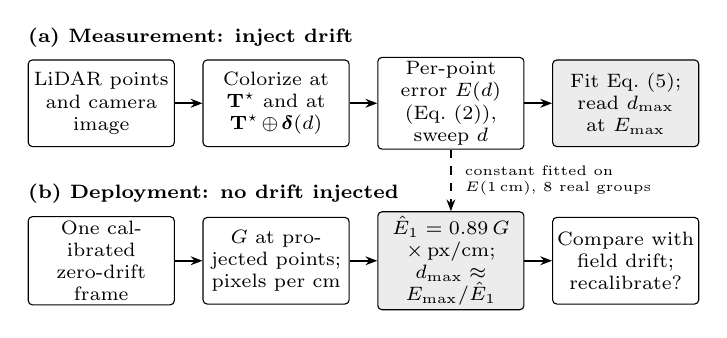
\begin{tikzpicture}[
  font=\scriptsize,
  box/.style={draw, rounded corners=1.5pt, align=center, inner sep=1.5pt,
              text width=17.5mm, minimum height=11mm},
  hl/.style={box, fill=gray!15},
  arr/.style={-{Stealth[length=1.5mm]}, semithick},
  lab/.style={font=\scriptsize\bfseries, anchor=south west, inner sep=0pt}]
\def\dx{22.2mm}
% ---------- (a) measurement ----------
\node[box] (a1) at (0,0) {LiDAR points\\and camera image};
\node[box] (a2) at (\dx,0) {Colorize at $\mathbf{T}^\star$ and at $\mathbf{T}^\star\!\oplus\!\boldsymbol{\delta}(d)$};
\node[box] (a3) at (2*\dx,0) {Per-point error $E(d)$ (Eq.~(2)), sweep $d$};
\node[hl]  (a4) at (3*\dx,0) {Fit Eq.~(5);\\read $d_{\max}$ at $E_{\max}$};
\foreach \i/\j in {a1/a2,a2/a3,a3/a4} \draw[arr] (\i) -- (\j);
\node[lab] at ($(a1.north west)+(0,1.5mm)$) {(a) Measurement: inject drift};
% ---------- (b) deployment ----------
\node[box] (b1) at (0,-20mm) {One calibrated zero-drift frame};
\node[box] (b2) at (\dx,-20mm) {$G$ at projected points; pixels per cm};
\node[hl]  (b3) at (2*\dx,-20mm) {\mbox{$\hat E_1=0.89\,G$}\\\mbox{$\times$\,px/cm;}\\\mbox{$d_{\max}\approx$}\\\mbox{$E_{\max}/\hat E_1$}};
\node[box] (b4) at (3*\dx,-20mm) {Compare with field drift; recalibrate?};
\foreach \i/\j in {b1/b2,b2/b3,b3/b4} \draw[arr] (\i) -- (\j);
\node[lab] at ($(b1.north west)+(0,1.5mm)$) {(b) Deployment: no drift injected};
% the constant of (b) is fitted on the measured error at 1 cm in (a)
\draw[arr, dashed] (a3.south) -- node[right, font=\tiny, align=left, xshift=0.5mm]
  {constant fitted on\\$E(1\,\mathrm{cm})$, 8 real groups} (b3.north);
\end{tikzpicture}
\end{document}
